\documentclass[]{article}

% ------
% Fonts and typesetting settings
\usepackage[sc]{mathpazo}
\usepackage[T1]{fontenc}
\linespread{1.05} % Palatino needs more space between lines
\usepackage{microtype}
\usepackage{amsmath}

% ------
% Page layout
\usepackage[hmarginratio=1:1,top=30mm,bottom=30mm,columnsep=20pt]{geometry}
\usepackage[font=it]{caption}
\usepackage{paralist}
%\usepackage{multicol}

\usepackage{graphicx}
\usepackage{color}
\usepackage{tabularx}

%\usepackage{wrapfig}

\usepackage{capt-of}

% \usepackage[ngerman]{babel}

% ------
% Lettrines
\usepackage{lettrine}

% ------
% Abstract
\usepackage{abstract}
	\renewcommand{\abstractnamefont}{\normalfont\bfseries}
	\renewcommand{\abstracttextfont}{\normalfont\small\itshape}


% ------
% Titling (section/subsection)
\usepackage{titlesec}
\renewcommand\thesection{\Roman{section}}
\titleformat{\section}[block]{\large\scshape\centering}{\thesection.}{1em}{}


% ------
% Header/footer
\usepackage{fancyhdr}
	\pagestyle{fancy}
	\fancyhead{}
	\fancyfoot{}
	\fancyhead[C]{Post-quantum cryptography $\bullet$ Winter 2018/19 $\bullet$ RheinMain University of Applied Sciences}
	\fancyfoot[RO,LE]{\thepage}


% ------
% Maketitle metadata
\title{\vspace{-7mm}%
	\fontsize{24pt}{10pt}\selectfont
	\textbf{Re-implementation of the Picnic signaturescheme in Python}
	}	
\author{%
	\large
	\textsc{Thorsten Knoll} \\[2mm]
	\normalsize	info@thorstenknoll.de \\[2mm]
	\normalsize March, 2019
	%\vspace{-5mm}
	}
\date{}

\usepackage[utf8]{inputenc}

\usepackage{hyperref}

%%%%%%%%%%%%%%%%%%%%%%%%
\begin{document}

\maketitle
\thispagestyle{fancy}

%\begin{abstract}
%\noindent Abstract goes here
%\end{abstract}

\section{Introduction}
\subsection{Post-quantum cryptography, NIST and Picnic}
Quantum computers are experiencing fast development and seem to be available within a timeframe of the next few decades. One of their properties will be to break huge parts of modern cryptography. Especially the discrete logarithm and prime-factorisation loose their trapdoor funcionality in regards to the efficient quantum algorithms from Grover and Shor. Therefore the need for new cryptographic algorithms arises, beeing save in regards to the availability of quantum computers. This field of research goes with the name "Post-quantum cryptography" (PQC). The american National Institute of Standards and Technology (NIST) called out a challenge to find the next PQC standards. This challenge is in round two of three at the time of writing this document. 69 submissions from round one were reduced to 26 candidates in round two of the challenge. These 26 candidates got announced by NIST not long ago at the end of january 2019. One of the submissions surviving the first round is the Picnic signaturescheme.\\ \\
NIST PQC page: \url{https://csrc.nist.gov/Projects/Post-Quantum-Cryptography} 
\subsection{Evaluation and reviews}
69 submissions is quite a huge amount in terms of reviewing and evaluating them. Additionaly PQC is a new field of research with a history not much longer than a decade. Cryptographers (and -analysts) are working intense on creating, evaluating, reviewing and breaking PQC algorithms. The state of PQC is that every litte step helps towards the goal of having secure PCQ algorithms. At RheinMain University of Applied Sciences (HSRM) the Master Students in Computer Science found together in a research course to participate in this process. This re-implementation is part of this efford.
\subsection{Goals: Learning Picnic (and LowMC)}
The sole purpose of this re-implementation is learning and understanding the Picnic algorithm and it's underlying zero-knowledge proof system. The goals are to provide an "easy to read and understand" codebase in a high-level language (Python) and make it a little easier to follow and learn the designprinciples of Picnic. The execution of Python-Picnic is awefull slow compared to the reference implementations in C. It is very unlikely that this will ever reach a usable state for production. Additionaly the code is not reviewed by anyone but the author and is surely not secure for productive use. But it may help to understand Picnic.\\ \\
On the way to understand Picnic, another algorithm must be understood too. That is the LowMC blockcipher. There are two main parts in Picnic, where LowMC plays a major role. Firstly the derivation of the public key is a LowMC encryption of the Picnic private key. Secondly each Picnic zero-knowledge round is a modified LowMC encryption, fitted into a Multi-Party-Computation (MPC) scheme. In the following description of the implementations we start with LowMC for that reason.
\subsection{Reference documents and implementations by the Picnic Team}
The original publications and reference implementations (in C) are available at: \\ \\
Microsoft Picnic projectpage: \url{https://www.microsoft.com/en-us/research/project/picnic/}\\
Microsoft Picnic Github: \url{https://github.com/Microsoft/Picnic}
\subsection{Re-implementations in Python}
These re-implementations in Python follow the original MIT Licenses and are public available at:\\ \\
LowMC in Python: \url{https://github.com/ThorKn/Python-LowMC}\\
Picnic in Python: \url{https://github.com/ThorKn/Python-Picnic}\\ \\
Installation and usage instructions are given inside the projects \texttt{README} files. This \texttt{PDF} can be found inside the \texttt{Python-Picnic} project in the \texttt{docs} folder.
\section{LowMC}
\subsection{Idea and overview}
Picnic makes intense use of the LowMC algorithm. Therefore we start with LowMC before hoping over to Picnic. A standalone LowMC Python-implementation got build as a starting point to understand Picnic. That is why there is a own Github project under the name \texttt{"Python-LowMC"}.\\ \\ 
LowMC is a blockcipher in a roundbased construction scheme like many other blockciphers. The name is an abbreviation for "Low multiplicative complexity". XOR in GF2 is a linear operation (ADD), while the multiplication (AND) in GF2 is a non-linear operation (Figure \ref{fig:gates}). LowMC tries to keep the count of AND operations as low as possible while still maintaining a given security level (L1, L3, L5). Additionaly LowMC is also designed to keep the AND-depth low. That means most AND operations could be done in parallel.\\
\begin{figure}[htbp]
\center
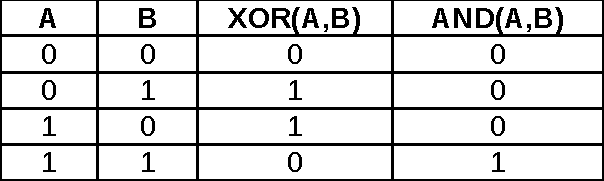
\includegraphics[width=0.35\textwidth]{pics/gates.pdf}
\caption{Linear and non-linear operations}
\label{fig:gates}
\end{figure}\\
Figure \ref{fig:lowmcscheme} shows the roundbased scheme of LowMC. Only the sbox part of the algorithm uses multiplications (ANDs). The other parts strictly contain only linear operations. From a mathematical point of view the XOR is a bijective function and the multiplications (ANDs) in GF2 are not bijective. Therefore the sboxes are the only not bijective part in LowMC. That is the reason for choosing LowMC in Picnic and it keeps the signature lengths smaller than with other blockciphers. We'll see how this is achieved with the Picnic implementation later on. 
\begin{figure}[htbp]
\center
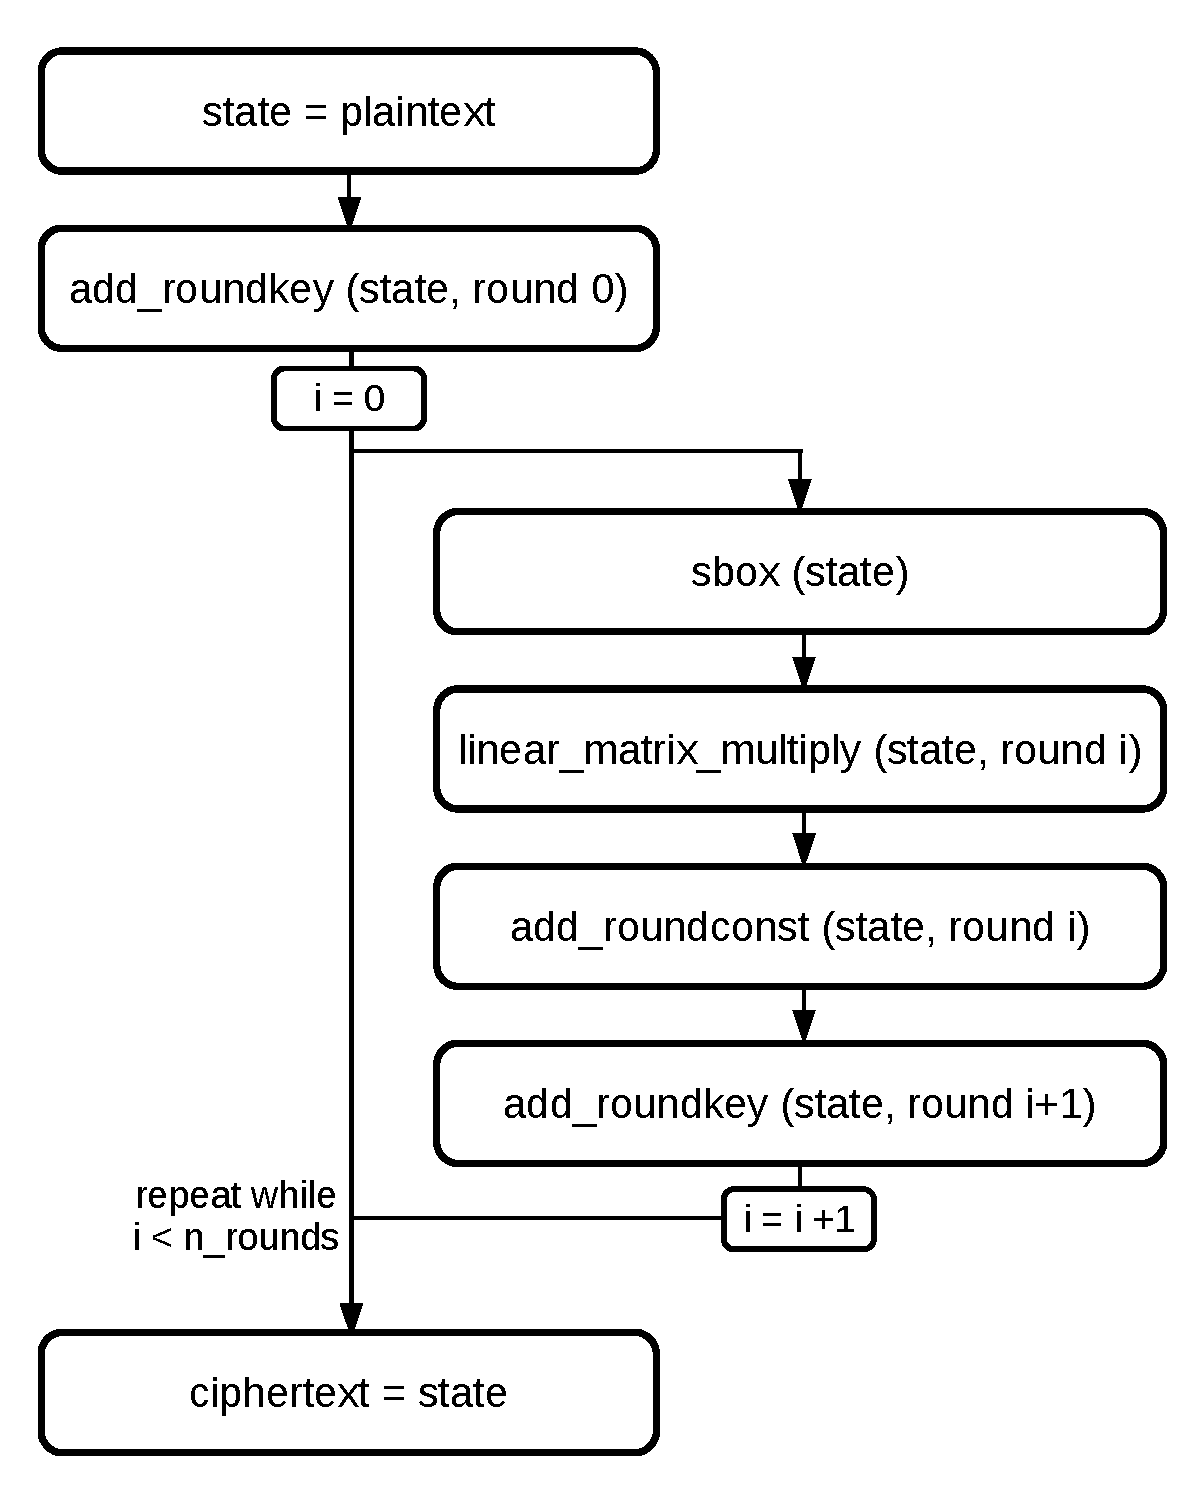
\includegraphics[width=0.5\textwidth]{pics/lowmc_scheme.pdf}
\caption{LowMC scheme}
\label{fig:lowmcscheme}
\end{figure}
\subsection{Pre-calculated constants}
The python program \texttt{generator.py} generates the files for all security levels with the following pre-calculated constants:
\begin{itemize}
\item{Linear layer matrices}
\item{Round constants}
\item{Roundkey matrices}
\end{itemize}
The generation of the constants-files is not mandatory for usage as the project contains them "ready to use". 
\subsection{Private functions}
\subsubsection{\texttt{\_\_apply\_sbox()}}
Sboxes are the only parts in LowMC, that contain multiplications in GF2 (ANDs). A fixed number of sboxes is applied to the state. Each sbox substitutes 3 Bit of the original state through a fixed substitution scheme. Let $a$, $b$ and $c$ be three bits in the state. Then $a'$, $b'$ and $c'$ get computed by:
\newpage
\[a' = a \oplus b \cdot c\]
\[b' = a \oplus b \oplus a \cdot c\]
\[c' = a \oplus b \oplus c \oplus a \cdot b\]
Where $\oplus$ is XOR and $\cdot$ is AND. So each 3-Bit sbox contains exactly 3 multiplications (ANDs). The security level (L1, L3, L5) defines the number of 3-Bit sboxes ($n$) per LowMC-round as shown in figure \ref{fig:sboxes}. The surplus Bits in the state get no substitution, shown on the right of the figure. The total number of multiplications for a complete encryption in LowMC sums up to $3 * n * rounds$. In example for security level L1 this calculates to $3 * 10 * 20 = 600$ ANDs.\\
\begin{figure}[htbp]
\center
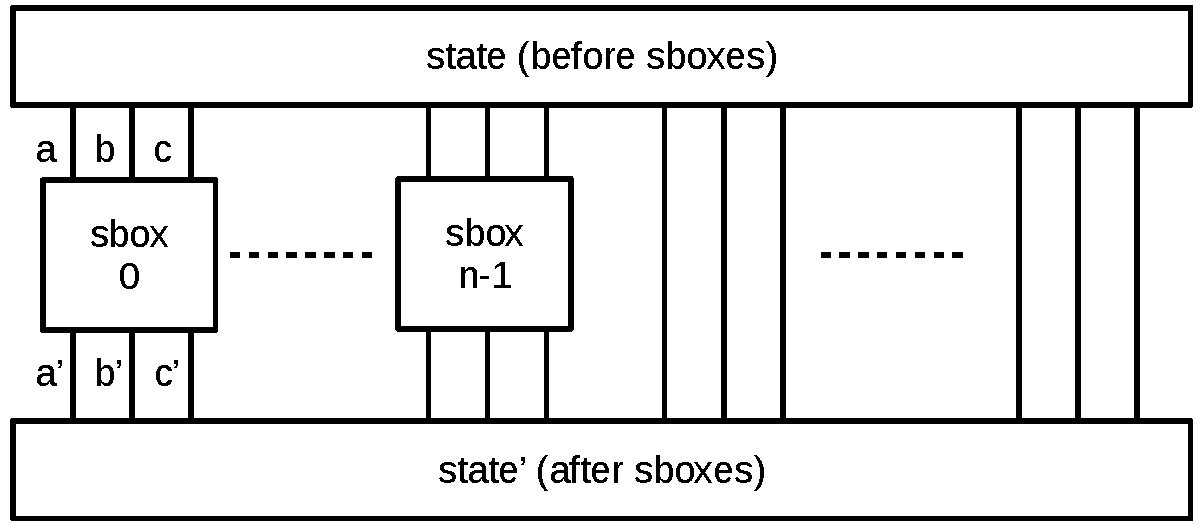
\includegraphics[width=0.5\textwidth]{pics/sboxes.pdf}
\caption{Sboxes per LowMC round}
\label{fig:sboxes}
\end{figure}\\
The function applies the sboxes to a state in memory and has no parameters and no returns. The actual state is stored in the private variable \texttt{self.\_\_state}. The sboxes are stored as a list (you can imagine it as a lookup-table) in the private variable \texttt{self.\_\_sbox}.
\subsubsection{\texttt{\_\_multiply\_with\_lin\_mat(round)}}
The state gets matrix multiplied with the constant and pre-calculated linear matrix. This contains only linear operations.
\subsubsection{\texttt{Add roundconstant}}
This needs no seperate function. It is a one-line operation with XOR on the state and therefore contains only linear operations.
\subsubsection{\texttt{\_\_key\_addition(round)}}
For XOR'ing the roundkey to the state the roundkey must be derived first. This is done by a matrix multiplication of the private key and the constant, pre-calculated roundkey-matrix. Again this only contains linear operations. 
\subsubsection{\texttt{Decryption functions}}
The decryption works pretty much the whole encryption way backwards. For the matrix multiplications their inverse matrices are needed. They get calculated within the constructor of the LowMC class and stored in seperate, private variables. The neccessary functions are named like the ones for encryption but with a \texttt{\_inv} appended to their names. The same rule applies for the names of their private variables.
\subsection{Public functions (API)}
\subsubsection{\texttt{LowMC(Security level) - Constructor}}
Constrcuts an object of LowMC with the parameters regarding to the security level. The following security levels are available and shall be given to the constructor as strings: "picnic-L1", "picnic-L3" and "picnic-L5". The fitting file with the constants must be in the project directory and gets read (see Pre-calculated constants). The constants from the file get stored in the private variables \texttt{self.\_\_lin\_layer}, \texttt{self.\_\_round\_consts} and \texttt{self.\_\_round\_key\_mats}.
\subsubsection{\texttt{generate\_priv\_key()}}
Generates a private key of the length specified within the security level. The private key is stored in the private variable \texttt{self.\_\_priv\_key}. The CSPRNG from the python package \texttt{os} is used (\texttt{os.urandom(bytelength)}).
\subsubsection{\texttt{set\_priv\_key(priv\_key)}}
Instead of generating the private key, it can also be set by giving a bytearry to this function. The bytearray must match the specified keylength from the security level.
\subsubsection{\texttt{encrypt(plaintext)}}
Encrypts a plaintext and returns the ciphertext. The plaintext length must match the specified blocksize length (security level) and must be given as a bytearray to the function. The ciphertext is returned as a bytearray of the same length. Before using this function a private key must be set (or generated).
\subsubsection{\texttt{decrypt(ciphertext)}}
Decrypts a ciphtertext and returns the plaintext. The ciphertext length must match the specified blocksize length (security level) and must be given as a bytearray to the function. The plaintext is returned as a bytearray of the same length. Before using this function a private key must be set (or generated).
\subsection{Testvectors}
The repository contains the python file \texttt{test\_lowmc.py}. One can simply run this and nine different testvectors get executed on the implementation. Three vectors for each security level. This testfile is also a good starting point to see how the implementation can be used.
\subsection{Prerequisites}
The code is tested with Ubuntu 16.04 LTS and Python3.6. The package "BitVector" for python is required. It is recommended to use a virtual environment for Python, like \texttt{virtualenv}. In (very) short lines:\\
\texttt{virtualenv --p /usr/bin/python3.6 myvenv}\\
\texttt{source /path\_to\_myvenv/bin/activate}\\
\texttt{<myvenv>pip install BitVector}\\
\texttt{<myvenv>python test\_lowmc.py}\\
\section{Picnic}

\bibliographystyle{unsrt}
\bibliography{}



\end{document}
